\documentclass{beamer}
\mode<presentation>
{ \usetheme{boxes} }

\usepackage{times}
\usepackage{graphicx}
\usepackage[backend=bibtex]{biblatex}
\usepackage{verbatim}
% \addbibresourse{an_introduction_to_dogen.bib}

\title{Using Watertight Polygon Meshes for Neuronal Morphology Representation}
\author{
  \texorpdfstring
      {\href{mailto:marco.craveiro@gmail.com}{Marco Craveiro}}
      {Marco Craveiro}
}
\date{\today}

\AtBeginSection[]
{
  \begin{frame}<beamer>
    \frametitle{Outline}
    \tableofcontents[currentsection]
  \end{frame}
}

\bibliography{watertight}

\begin{document}

\begin{frame}
\titlepage
\end{frame}

\begin{frame}
\frametitle{Outline}
\begin{itemize}
\item Microscopy and Computational Neuroscience
\pause
\item SWC format
\pause
\item Polygon meshes
\pause
\item Questions / Discussion
\end{itemize}
\end{frame}

\begin{frame}
\frametitle{Microscopy and computational neuroscience}

\begin{itemize}

\item Microscopy is an important source of data on neuron morphology.
\pause
\item There are many kinds of microscopy (EM, Optical, etc.) and the
  field has evolved dramatically over the last few years.
\pause
\item The latest generation Electron Microscopes can generate
  terabytes of data at very high resolution (1 nm or higher).
\pause
\item At this resolution it is possible to see very small
  sub-structures inside of the neuron, which are important for
  morphometric work.

\end{itemize}

\end{frame}

\begin{frame}
\frametitle{Microscopy and computational neuroscience}

\begin{figure}[H]
    \centering
    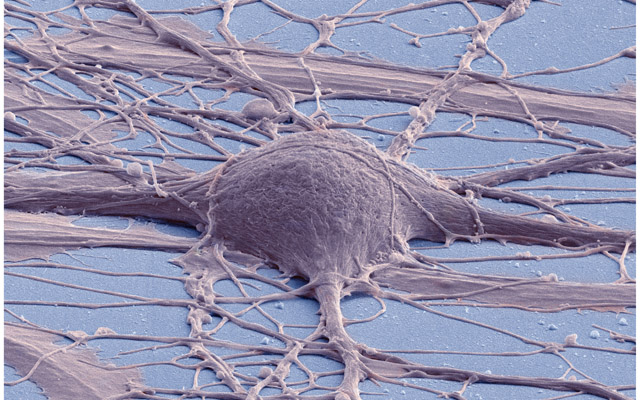
\includegraphics[scale=2]{../blog/images/2014_06_26_human_ipsc_derived_neuron_deerinck}
    \caption{Human neuron from SEM (Scanning Electron Microscope) micrograph. Source: New Reprogramming Method Makes Better Stem Cells
      \url{http://ucsdnews.ucsd.edu/pressrelease/new_reprogramming_method_makes_better_stem_cells}.}
    \label{fig:3d_neuron}
\end{figure}

\end{frame}

\begin{frame}
\frametitle{Microscopy and computational neuroscience}

\begin{itemize}
\item The data generated by the microscopes cannot be used
  directly.
\pause
\item One must first perform recognition of the objects in the
  micrographs. This is known as \emph{segmentation} and
  \emph{reconstruction}.
\pause
\item Until recently these tasks were performed manually. Experienced
  lab technicians would identify and measure all of the structures in
  the neuron. This is a low-resolution/high-error process.
\pause
\item Recently Machine Learning has been applied to the task with
  success.
\end{itemize}

\end{frame}

\begin{frame}
\frametitle{Microscopy and computational neuroscience}

Sample micrograph from a stack. Left-hand side shows the original
micrograph; right-hand side shows the result of processing it with
machine learning.

\begin{figure}[H]
    \centering
    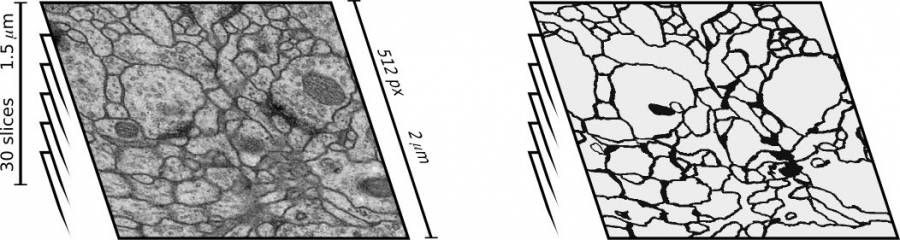
\includegraphics[scale=0.3]{../blog/images/biomed-neurons}
    \caption{Source: Deep Neural Networks Segment Neuronal Membranes in Electron Microscopy Images
      \url{http://papers.nips.cc/paper/4741-deep-neural-networks-segment-neuronal-membranes-in-electron-microscopy-images.pdf}.}
    \label{fig:stack}
\end{figure}

\end{frame}

\begin{frame}
\frametitle{Microscopy and computational neuroscience}

Reconstruction of 3D structures from a stack.

\begin{figure}[H]
    \centering
    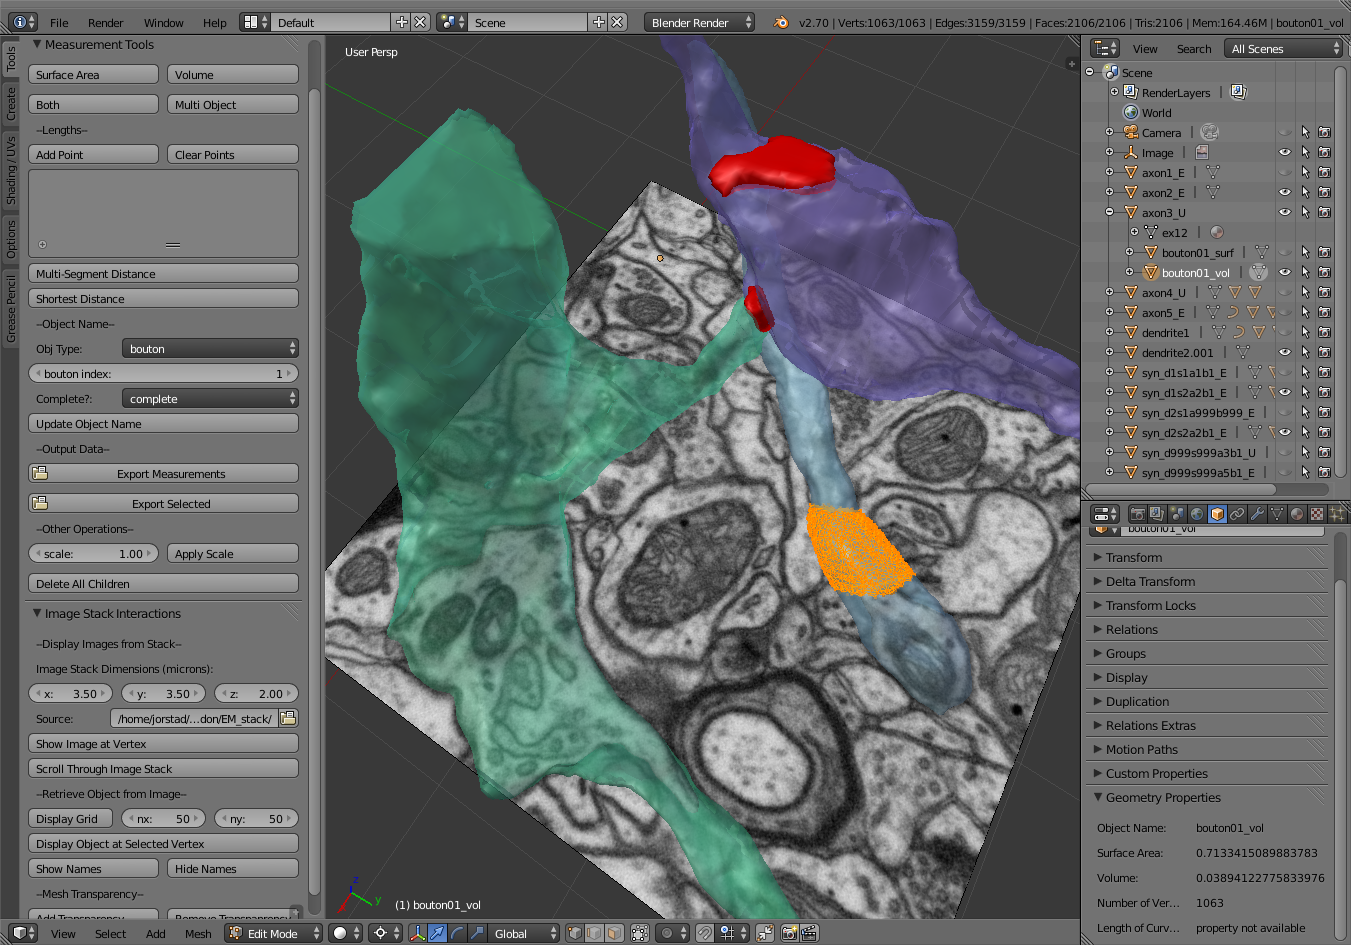
\includegraphics[scale=0.2]{../blog/images/NeuroMorph_screenshot.png}
    \caption{Source: Segmented anisotropic ssTEM dataset of neural tissue
      \url{http://figshare.com/articles/Segmented_anisotropic_ssTEM_dataset_of_neural_tissue/856713}.}
    \label{fig:3d_stack}
\end{figure}

\end{frame}

\begin{frame}
\frametitle{Microscopy and computational neuroscience}

Allen Brain Atlas user interface browsing a micrograph in a stack,
with corresponding reconstruction.

\begin{figure}[H]
    \centering
    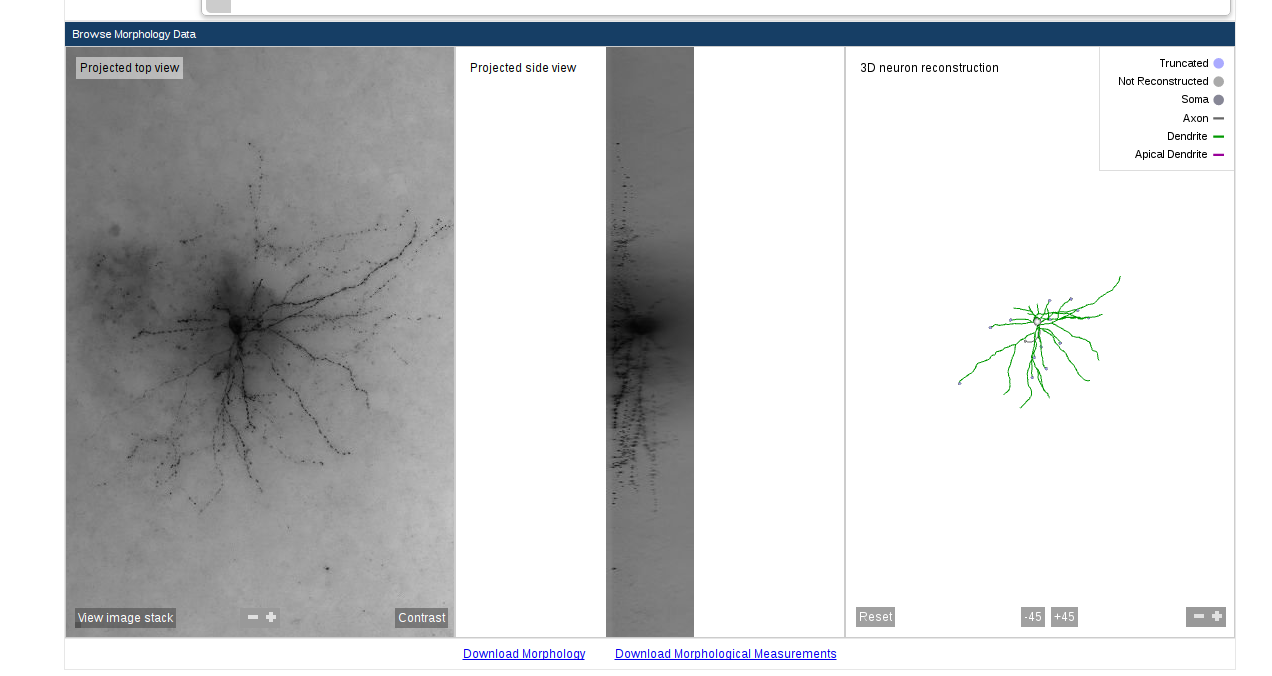
\includegraphics[scale=0.2]{../blog/images/allen_brain_atlas_primary_visual.png}
    \caption{Source: Allen Brain Atlas, Primary visual area, layer 5.
      \url{http://celltypes.brain-map.org/mouse/experiment/morphology/469610831}.}
    \label{fig:3d_stack}
\end{figure}

\end{frame}

\begin{frame}[fragile]
\frametitle{SWC}

\begin{itemize}

\item \emph{De facto} standard for storing morphology data.
\pause
\item As seen on Felix's presentation, the data is stored as a tree.
\pause
\item The internal format is a set of frusta (truncated cones),
  connected together in a parent and child relationship.
\pause
\item Powerful: morphometric work can be carried out from this simple
  tree representation, as per the functions provided by TREES and
  TREES2. Also useful for electrophysiology models, etc.
\pause
\end{itemize}

\begin{verbatim}
# id,type,x,y,z,r,pid
1 1 305.7912 312.7696 31.92 8.059 -1
2 2 307.4752 319.1016 31.9197 0.1144 1
3 2 307.7989 320.1896 31.8424 0.1731 2
5 2 309.0413 322.0349 31.7724 0.2652 4
...
\end{verbatim}
\end{frame}

\begin{frame}
\frametitle{SWC}

SWC is a good format which has withstood the test of time, but has
some important shortcomings.
\pause

\begin{itemize}
\item Microscopy has improved dramatically but the resolution SWC
  provides is frusta: all of the high-resolution detail is lost in the
  final representation.
\pause
\item Loss of detail is applicable to both soma and the dendrites: the
  soma is represented as a sphere or a similar solid; the dendrites
  may miss dendritic spines altogether or have very inaccurate
  representations.
\pause
\item SWC was designed in the nineties, where computer capacity (CPU,
  storage, network bandwidth, etc) was a fraction of what we have
  today. We no longer have the same constraints.
\pause
\item SWC provides limited extensibility for annotation and tagging
  of objects, including the reconstruction itself.
\end{itemize}

\end{frame}

\begin{frame}
\frametitle{SWC}

\begin{itemize}
\item For certain uses the loss of resolution may not have a
  significant impact: ``in electro-physiological models, the space
  constants are likely larger than geometric ambiguities''; however
  ``these still show up as discrepancies in voltage
  traces.''\cite{mcdougal2013water}.
\pause
\item In other cases it may be of great importance:
  \begin{itemize}
  \item Low-resolution is ``unsuitable for multi-scale models that
    also involve three-dimensional reaction-diffusion, as such models
    have smaller space constants.''\cite{mcdougal2013water}
  \pause
  \item Morphometric work would benefit from a higher resolution. For
    example, dendritic spine alterations are important in studies of
    Alzheimer's disease \cite{smith2009reversal}.
  \pause
  \end{itemize}
\item There may be new scientific questions that will only be posed
  when more accurate reconstructions are available.
\pause
\end{itemize}

\end{frame}

\begin{frame}
\frametitle{SWC}

Example of measurements one may want to perform on a dendrite.

\begin{figure}[H]
    \centering
    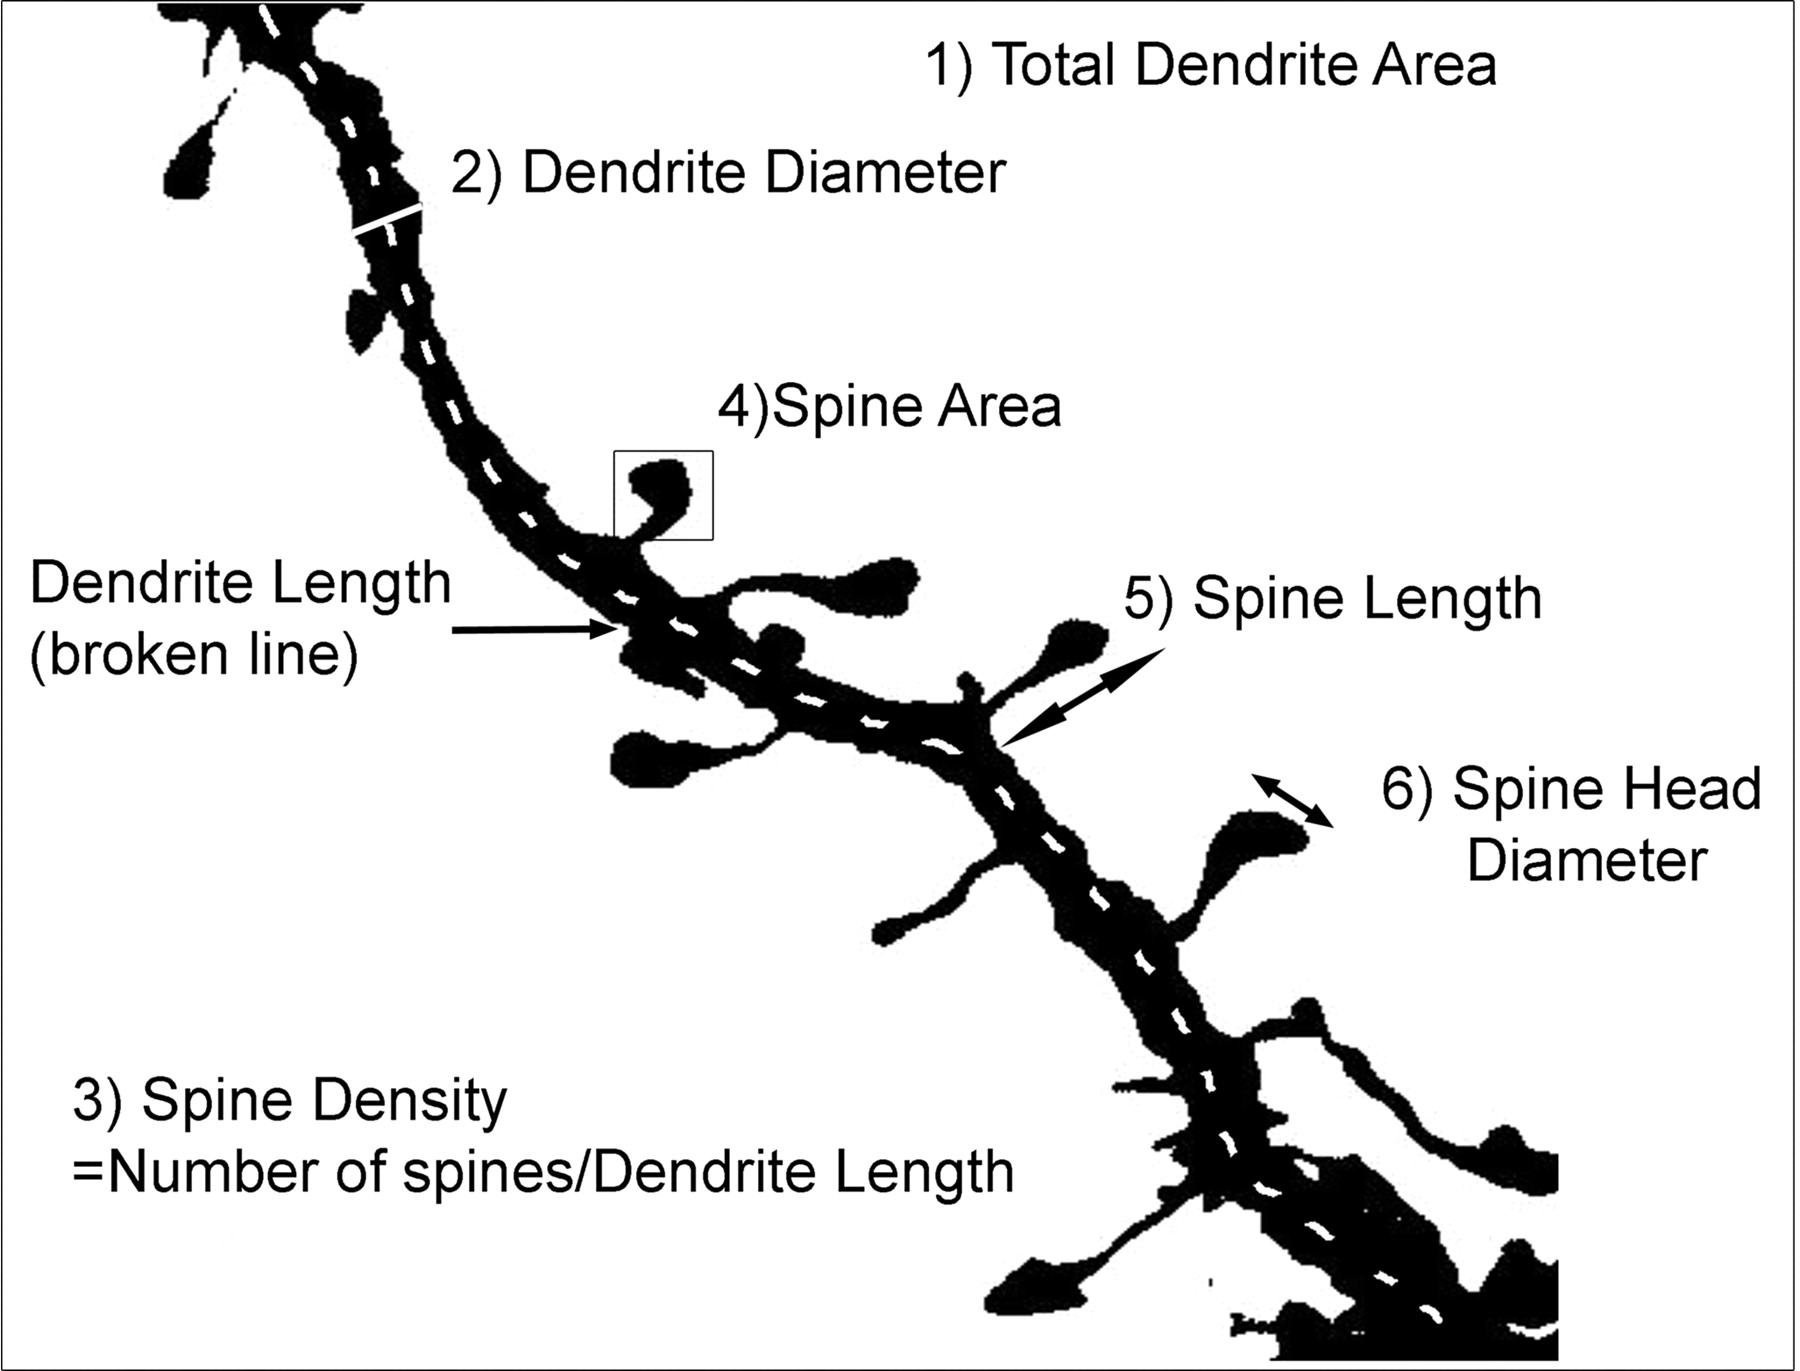
\includegraphics[scale=0.1]{../blog/images/F1_large}
    \caption{Source: Reversal of long-term dendritic spine alterations in Alzheimer disease models.
      \url{http://www.pnas.org/content/106/39/16877.abstract}.}
    \label{fig:morphometry}
\end{figure}

\end{frame}

\begin{frame}
\frametitle{Polygon meshes}

Our approach is to use polygon meshes to provide more accurate
representations of neuronal morphologies.

\pause

\begin{itemize}
\item A polygon mesh is composed of large numbers of simple polygons
  such as triangles or quads. These are stitched together to represent
  a surface.
\pause
\item In an ideal world one would want to use volumetric meshes, which
  stitch together polyhedra to fill the represented volume. However,
  at present we are only looking at surface meshes.
\pause
\item We have additional requirements on surface meshes in order for
  them to be applicable to all use cases~--- morphometry,
  reaction-diffusion, electrophysiology, etc~--- which are not needed
  for other uses such as computer graphics/games.
\end{itemize}

\end{frame}

\begin{frame}
\frametitle{Polygon meshes}

Polygon meshes are popular:

\pause

\begin{itemize}
\item The popularity of Computer Graphics and 3D Printing means that
  there are many libraries, packages and applications to choose
  from. There are also a number of file formats for meshes (OFF, STL,
  etc).
\pause
\item We want to define our own file format since we want to add
  annotations specific to neuroscience, but we also want to reuse
  existing mesh formats.
\end{itemize}

\end{frame}

\begin{frame}
\frametitle{Polygon meshes}

``Water-tight membranes from neuronal morphology files'':

\begin{itemize}
\item This is not a new idea. In particular, McDougal, Hines and
  Lytton wrote a paper\cite{mcdougal2013water} where they describe an
  approach to convert SWC files into water-tight meshes.
\pause
\item It is of course not possible to reconstruct the neuron's full
  shape from point and diameter data, the generated meshes are still
  useful because they define a plausible reconstruction without gaps
  and \emph{cul-de-sacs}.
\pause
\item Its a good starting point on the road to defining a mesh format
  because we can compare with the original SWC and there is a wealth
  of data available.
\pause
\item The end goal however is to use high-resolution microscopy data
  as an input to the mesh generation process.
\pause
\item Another possibility is computer generated neurons which are
  realistic.
\end{itemize}

\end{frame}

\begin{frame}
\frametitle{Polygon meshes}

McDougal et al. define the criteria for the generated meshes:

\begin{itemize}
\item They must be physically plausible: ``the same space cannot be
  occupied by different matter, the surface must not have holes and
  the surface must not lie inside of the
  neuron.''\cite{mcdougal2013water}
\pause
\item They must be biologically plausible: ``no portion of a dendrite
  must extend past its neighbour.''\cite{mcdougal2013water}
\end{itemize}

\end{frame}

\begin{frame}
\frametitle{Polygon meshes}

Meshes must be completely manifold or watertight. This is a very
important requirement.
\pause

\begin{itemize}
\item Mathematical understanding: Non-manifolded edges are a
  problem. These are are parts of a model where the dots have not been
  connected to create a polygon. A line, or even a plane, does not have
  dimensions in three separate directions (x, y, z).
\pause
\item Intuitive understanding: if one were to fill in a physical
  representation of the model with water, would it have leaks.
\end{itemize}

\end{frame}

\begin{frame}
\frametitle{Polygon meshes}

The mesh generation process:

\begin{itemize}
\item First step: ``fix'' the SWC file, looking for
  inconsistencies such as missing parents, points with the same
  position on the plane and so on.
\pause
\item Second step: convert SWC into a CSG (Constructive Solid Geometry)
  representation. This has a number of primitives, defined by implicit
  functions. At this stage we can deal with join problems.
\pause
\item Third step: Convert the CSG representation into a mesh
  representation by polygonising/tessellating the CSG primitives. At
  this stage we can deal with affine transformations.
\pause
\item Forth step: Ensure the validity of the surface by using CTNG
  (Constructed Tesselated Neuronal Geometry), which removes parts of
  the surface that lie inside of it and ensures the generation of a
  consistent, continuous surface.
\end{itemize}

\end{frame}

\begin{frame}
\frametitle{Polygon meshes}

Progress:

\begin{itemize}
\item At present writing a C++ implementation of the processing
  pipeline using the Eigen and CGAL libraries.
\pause
\item Whilst there are many libraries available, a lot of glue code
  still has to be written. Coding has been slow/difficult because the
  domain is to mathematical.
\pause
\item Code is very CPU-intensive and will benefit from parallelism. It
  is being written so we can use a grid.
\pause
\item Once we have a basic pipeline working with a defective surface,
  we will implement CTNG and generate water-tight meshes.
\pause
\end{itemize}

\end{frame}


\begin{frame}
\frametitle{Questions?}

\end{frame}

\begin{frame}
  \printbibliography
\end{frame}

\end{document}
